\epigraph{\ttfamily
I like the little-known operator "-{}->", also know as "goes to."\\[\baselineskip]
Here's an example:\\[\baselineskip]
\#include <stdio.h>\\
int main()\\
\{\\
~~int x = 10;\\
~~while( x -{}-> 0 ) // x goes to 0\\
~~\{\\
~~~~printf("\%d ", x);\\
~~\}\\
\}%
}{--- \textup{comp.lang.c++.moderated}, Hidden Features and Dark Corners of C++/STL}

In \Cref{ch:syntacticproof} we introduced a class of loops for which termination can be shown with minimal information in a \emph{syntactic termination proof}. These proofs were obtained by leveraging locally available information about updates to a counter variable and the syntactic structure of the loop's exit predicates. Obviously, current techniques and tools are capable of handling more complicated cases. As we shall see in \Cref{ch:experimental}, \loopus{} can bound 79\% of the loops in the cBench benchmark suite, while only 37\% of all loops are syntactically terminating loops.

Formal methods-based techniques like \loopus{} usually achieve this wider coverage by considering a more complete representation of the program: The effect of statements is chained together, usually into a formula in classical logic that represents the whole program. Search for a property is then left to an off-the-shelf SAT or SMT solver. This approach is illustrated in \Cref{lst:ssa}, where the comments show an encoding of the C program in the first-order theories of equality and linear arithmetic.

\begin{listing}
    \begin{ccode}
int i = 0;      // $i_0 = 0,$
i++;            // $i_1 = i_0 + 1,$
if (i == 0) {   // $i_1 = 0 \rightarrow ($
    i--;        // $     i_2 = i_1 - 1$
} else {        // $), i_1 \ne 0 \rightarrow ($
    i++;        // $     i_2 = i_1 + 1$
}               // $),$
assert(i==2);   // $i_2 = 2$
    \end{ccode}
    \caption{A sample C program expressed as conjunction over equality and linear arithmetic.}
    \label{lst:ssa}.
\end{listing}

It is unreasonable to reimplement such an approach for our analysis, as it would basically make our tool \sloopy{} a tool that \emph{proves termination}, instead of a tool that \emph{efficiently determines difficulty to prove termination}. Instead, to express a superset of syntactically terminating loops we will exploit the fact that programmers follow patterns: Assume an at least slightly experienced programmer is asked to implement a subprogram that performs a task $n$ times. He will probably come up with program $P$, or some slight variation of the same basic pattern, even though infinitely many subprograms conforming to the same specification exist (e.g.\ illustrated in program $Q$ below).

\begin{center}
\begin{minipage}{.48\linewidth}
\begin{listing}[H]
\begin{ccode*}{linenos=false}
for (int i = 0; i < n; i++) {
    // perform task
}
\end{ccode*}
\caption{Example program $P$.}
\end{listing}
\end{minipage}
\hfill
\begin{minipage}{.48\linewidth}
\begin{listing}[H]
\begin{ccode*}{linenos=false}
int j = 3;
int *i = &j;
loop:
// perform task
*i = j-1;
j += 2;
if (3+n == **&i) ;
else goto loop;
\end{ccode*}
\caption{Example program $Q$.}
\end{listing}
\end{minipage}
\end{center}

If we can weaken syntactically terminating loops to describe such patterns in a way that leaves enough leeway to match a considerable amount of loops, but still captures the termination-related properties of syntactically terminating loops well, we have found our desired classification. Additionally, a classification with respect to these patterns can be used to guide the non-trivial decision where to apply and how to parametrize formal methods, as discussed in the introduction to this work. We describe \emph{simple loops}, a family of such patterns:

\section{Dimensions of Simple Loops}

As proposed, we derive simple loops from syntactically terminating loops. We do so by systematically weakening the constraints used to define syntactically terminating loops along three dimensions, allowing us to tweak how many features of this class are retained. We start by introducing these dimensions and then describe the family of all possible combinations along these dimensions.

\begin{figure}
\begin{minipage}{.38\linewidth}
    \begin{ccode}
for (int i = 0; ; i++) {
    if (i < 100) {
        if (i == 10) break;
    } else {
        if (i == 110) break;
    }
}
    \end{ccode}
\end{minipage}
\hfill
\begin{minipage}{.58\linewidth}
\begin{tikzpicture}[%
    ->,
    node distance=0.5,
    box/.style={draw, rectangle, align=center}
  ]
\node[box] (0) at (0,0) {\entry};
\node[box, below=of 0] (2) {[1]\\for (...; 1; ...)};
\node[box, below=of 2] (3) {[2]\\if (i < 100)};
\node[box, below left=of 3,xshift=0.5cm] (4) {[3]\\if (i == 10)};
\node[box, below right=of 3,xshift=-0.5cm] (5) {[5]\\if (i == 110)};
\node[box, below=of 3,yshift=-2cm] (6) {[6]\\i++};
\node[box, below=of 5,xshift=0.5cm,yshift=-1cm] (exit) {\exit};
\path (0) edge (2)
      (2) edge (3)
      (3) edge (4)
      (3) edge[dashed] (5)
      (4) edge[dashed] (6)
      (5) edge[dashed] (6)
      (6) edge[out=180, in=180, looseness=2] (2)
      (4) edge (exit)
      (5) edge (exit);
\end{tikzpicture}
\end{minipage}
\caption{A terminating loop for which our analysis cannot compute a syntactic termination proof because of non-local control flow.}
\label{fig:terminating_not_synt}
\end{figure}

\begin{description}
    \item[Control flow constraints] In \Cref{sec:control_flow}, we put a strong restriction on the control flow of syntactically terminating loops: The terminating block $b$ associated with a terminating predicate $P: assume(\mathlist{b, \exit})$ has to lie on each path through the loop. \Cref{fig:terminating_not_synt} illustrates a loop that terminates, but does not have a singleton terminating block on all paths:
        \begin{example}
            The loop shown in \Cref{fig:terminating_not_synt} counts \texttt{i} upwards from 0. When $i = 10$, the \texttt{if} statement in block [2] branches to block [3]. There, the \texttt{if} statement's condition evaluates to true, the \texttt{break} statement is executed and leaves the loop. However, because of the locality of our analysis, we cannot capture the interplay between block [2] and blocks [3] or [5], respectively. More formally, our path-insensitive analysis cannot decide that block [2] branches to block [3] when $i = 10$.
        \end{example}
        This lends itself to introduce the following heuristic instead: Given the set of all terminating blocks $T$, assume some terminating block in $t \in T$ associated with exit predicate $P$ is executed at some point when $P$ holds, thus terminating the loop. We give a formal definition:
    \begin{definition}
        Given a natural loop $L$, let predicate $tb: L \rightarrow \{\text{true}, \text{false}\}$ determine if its argument is a terminating block, i.e.\ $tb(b)$ if and only if $b$ is a terminating block. The three control flow constraints $\textsf{s}, \textsf{p}, \textsf{w}$ are defined as follows:
    \begin{align*}
        \textsf{p}&: \exists b \in L \ldotp \forall p \in paths(L) \ldotp tb(b) \land b \in p \\
        \textsf{s}&: \forall p \in paths(L) \ldotp \exists b \in L \ldotp tb(b) \land b \in p \\
        \textsf{w}&: \exists b \in L \ldotp tb(b)
    \end{align*}
    \end{definition}
    Intuitively, \textsf{p} requires a singleton terminating block that lies on each path, \textsf{s} requires some terminating block (not necessarily the same) on each path, and \textsf{w} merely requires existence of some terminating block.
    \item[Well-formedness constraints] As discussed in \Cref{sec:acc_inc}, we cannot fold non-constant increment values into the accumulated increment. However, often a symbolic delta will take sensible values, but again with our local, path-insensitive analysis we cannot establish those. In \Cref{lst:terminating_not_synt2} we illustrate such a terminating loop for which our analysis cannot establish a syntactic termination proof:

\begin{listing}
\begin{ccode}
int i = 0,
    D = 3;
while (i < 10) {
    i += D;
    D++;
}
\end{ccode}
\caption{A terminating loop for which our analysis cannot compute a syntactic termination proof because of non-constant increments.}
\label{lst:terminating_not_synt2}
\end{listing}

        \begin{example}
            The loop in \Cref{lst:terminating_not_synt2} increments \texttt{i} by the value of \texttt{D}. At line 3 we consecutively see the values 0, 3, 7, 12 for \texttt{i} -- at the last value iteration terminates. However, due to lack of contextual information about the value of \texttt{D} at line 4, we loose all information about the accumulated increment of \texttt{i}.
        \end{example}
        As above, we introduce a heuristic for this case: We decouple the termination property of exit predicates by not requiring the accumulated increment to imply eventual truth of the predicate:
    \begin{definition}
        Given a natural loop $L$ satisfying a control flow constraint $C$, let $B \subseteq L$ denote the minimal set of blocks needed to satisfy $C$. Let predicate $wp$ determine if its argument is a well-formed predicate, i.e. $wp(P)$ if and only if $P$ is a well-formed predicate (c.f.\ \Cref{def:wpred}). Let predicate $tp$ determine if its argument is a terminating predicate, i.e.\ $tp(P)$ if and only if $P$ is a terminating predicate (c.f.\ \Cref{def:tpred}). The two well-formedness constraints $\textsf{t}, \textsf{w}$ are defined as follows:
    \begin{align*}
        \textsf{t}&: \exists b \in B \ldotp tp(assume(b, \exit) \\
        \textsf{w}&: \exists b \in B \ldotp wp(assume(b, \exit) \\
    \end{align*}
    \end{definition}
    We extend the control flow constraint above to consider blocks of well-formed predicates instead of terminating blocks if the weaker constraint \textsf{w} is chosen.
    \item[Invariant bound constraints] As mentioned in \Cref{sec:term_pred}, we only consider linear inequalities in a single variable for our syntactic termination proof. Other subexpressions are checked to be loop-invariant. If we omit this check, we obtain a weaker constraint on the loop's behavior.
    \begin{definition}
        Let $L$ be a natural loop, and $V$ the set of variables that need to be checked for loop-invariance. Let predicate $inv: V \rightarrow \{\text{true}, \text{false}\}$ determine if its argument is loop-invariant, i.e. $inv(v)$ if and only if $v$ is loop-invariant in $L$. The two invariance constraints $\textsf{i}, \textsf{x}$ are defined as follows:
    \begin{align*}
        \textsf{i}&: \forall v \in V \ldotp inv(v) \\
        \textsf{x}&: \text{ true}
    \end{align*}
    \end{definition}
\end{description}

In addition to the previous three dimensions that derive loop classes from the constraints of syntactically terminating loops, we can restrict simple loops by intersecting them with any other loop class. We exemplarily do this for a structural loop class from \Cref{ch:structural}:

\begin{description}
    \item[Exit constraint] As discussed in \Cref{sec:class_cfg}, we can impose constraints of the number of exits. This is especially useful in conjunction with control flow constraints, e.g.\ we may only require a terminating block on some path, but enforce that this exit is the singleton exit from the loop. Additionally, in our experience (c.f.\ \Cref{sub:number_of_exits}) fewer exits are a strong indicator for low difficulty to compute a termination proof (as indicated by \loopus{}). This restriction can be achieved by intersecting the set of loops in some class $C$ and the set of loops with $n$ exits: $\mathcal{L}^C \cap \mathcal{L}^{E=n}$.
    \begin{definition}
        Let $L$ be a natural loop. The exit constraints $\textsf{1}, \textsf{*}$ are defined as $\textsf{1}: L \in \mathcal{L}^{E=1}$ and $\textsf{*}: \text{true}$.
    \end{definition}
\end{description}

\begin{definition}[Simple loop constraint]
A \emph{simple loop constraint} is a tuple $(N, C, I, W)$, where $N$ is an exit constraint, $C$ is a control flow constraint, $I$ is a loop-invariance constraint, and $W$ is a well-formedness constraint. A natural loop $L$ satisfies constraint $(N, C, I, W)$ if and only if all of $N, C, I, W$ are satisfied for $L$. $L$ is a simple loop $L \in \mathcal{L}^{simple(NCIW)}$ if and only if $L$ satisfies $(N, C, I, W)$.
\end{definition}

For a visual interpretation, consider \Cref{fig:simpleloopdim} showing the four categories above as independent dimensions. Moving away from the center along dimensions $C$, $I$, or $W$, we cover additional loops at the expense of losing soundness. Along dimension $N$, we do not trade soundness, but allow tweaking of the loop's simplicity via a structural measure. One may also leave the $N$ dimension uninstantiated, thus covering loops with any number of exits.

\begin{figure}
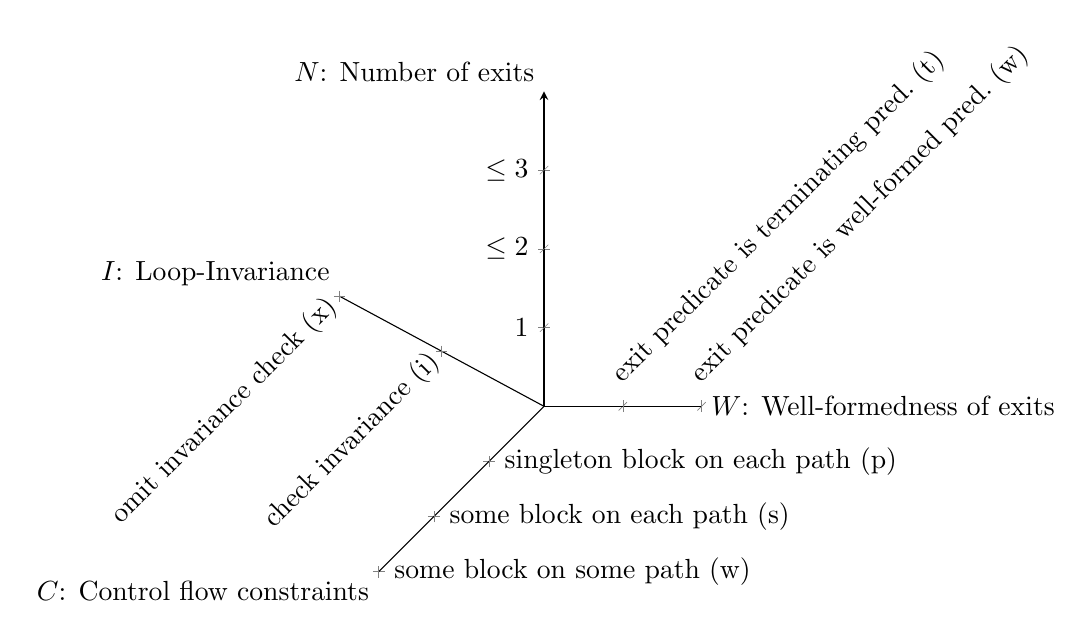
\begin{tikzpicture}
    \begin{axis}[clip=false,axis lines=center,
        x axis line style=-,
        y axis line style=-,
        x={(-0.7cm,-0.7cm)}, y={(1cm,0cm)}, z={(0cm,1cm)},
        xmin=0, xmax=3, ymin=0, ymax=2, zmin=0, zmax=4,
        xlabel={$C$: Control flow constraints},
        xlabel style={anchor=north east},
        ylabel={$W$: Well-formedness of exits},
        ylabel style={anchor=west},
        zlabel={$N$: Number of exits},
        zlabel style={anchor=south east},
        x tick label style={anchor=west,xshift=1ex},
        z tick label style={anchor=east},
        xtick={1,2,3},
        xticklabels={singleton block on each path (p), some block on each path (s), some block on some path (w)},
        y tick label style={rotate=45,anchor=south west},
        ytick={1,2,3},
        yticklabels={exit predicate is terminating pred.\ (t), exit predicate is well-formed pred.\ (w)},
        ztick={1,2,3},
        zticklabels={$1$, $\le 2$, $\le 3$},
]
    \draw (axis cs:0,0) -- (axis cs:-2,-4);
    \node[rotate=45, anchor=east] at (axis cs:-1,-2) {check invariance (i)};
    \node[rotate=45, anchor=east] at (axis cs:-2,-4) {omit invariance check (x)};
    \node[anchor=south east] at (axis cs:-2,-4) {$I$: Loop-Invariance};

\addplot[mark options={gray, very thin}, only marks, mark=+] coordinates { (-1,-2) };
\addplot[mark options={gray, very thin}, only marks, mark=+] coordinates { (-2,-4) };

    \end{axis}
\end{tikzpicture}
\caption{Four dimensions of simple loops.}
\label{fig:simpleloopdim}
\end{figure}

To aid communication about simple loops, we introduce a naming scheme for the classes of the simple loop family: Loops with a single exit ($N = \textsf{1}$) are referred to as \emph{single-exit loops}. Depending on the control flow constraint, we have \emph{proved-cf}, \emph{strong-cf}, \emph{weak-cf loops}, if they have a singleton block on each path ($C = \textsf{p}$), some block on each path ($C = \textsf{s}$), some block on some path ($C = \textsf{w}$), respectively. Loops fulfilling the loop-invariance restriction ($C = \textsf{i}$) are \emph{invariant loops}. If the increment implies termination ($W = \textsf{t}$) we speak of \emph{terminating loops}. If we mitigate this constraint to a form of syntactic well-formedness ($W = \textsf{w}$), we speak of \emph{well-formed loops}. This naming scheme is summarized in \Cref{tab:simpleloopnames}.

\begin{table}
    \begin{tabular}{ll}
    $N = 1$   & single-exit  \\ \hline
    $C = \text{p}$ & proved-cf \\
    $C = \text{s}$ & strong-cf \\
    $C = \text{w}$ & weak-cf \\ \hline
    $I = \text{i}$ & invariant \\ \hline
    $W = \text{t}$ & terminating  \\
    $W = \text{w}$ & well-formed  \\
    \end{tabular}
    \caption{Naming scheme for simple loops.}
    \label{tab:simpleloopnames}
\end{table}

Note that the class $\mathcal{L}^{simple(\textsf{*pit})}$ is the class of syntactically terminating loops introduced in \Cref{ch:syntacticproof}: $\mathcal{L}^{simple(\textsf{*pit})}$ = $\mathcal{L}^{ST}$. In addition to $\mathcal{L}^{ST}$, we obtain the eleven additional simple loop classes listed in \Cref{tab:simple_loop_classes} and the corresponding single-exit classes $\mathcal{L}^{simple(\textsf{1}CIW)}$.

\begin{table}
\begin{tabular}{Hll}\toprule
    Constraint & Class & Name \\ \midrule
    $(C = \text{p}, I = \text{i}, W = \text{t})$ & $\mathcal{L}^{simple(\text{*pit})}$ & syntactically terminating \\
    $(C = \text{s}, I = \text{i}, W = \text{t})$ & $\mathcal{L}^{simple(\text{*sit})}$ & (any-exit) strong-cf invariant terminating \\
    $(C = \text{w}, I = \text{i}, W = \text{t})$ & $\mathcal{L}^{simple(\text{*wit})}$ & (any-exit) weak-cf invariant terminating \\
    $(C = \text{p}, I = \text{i}, W = \text{w})$ & $\mathcal{L}^{simple(\text{*piw})}$ & (any-exit) proved-cf invariant well-formed \\
    $(C = \text{s}, I = \text{i}, W = \text{w})$ & $\mathcal{L}^{simple(\text{*siw})}$ & (any-exit) strong-cf invariant well-formed \\
    $(C = \text{w}, I = \text{i}, W = \text{w})$ & $\mathcal{L}^{simple(\text{*wiw})}$ & (any-exit) weak-cf invariant well-formed \\ \midrule
    $(C = \text{p}, I = \text{x}, W = \text{t})$ & $\mathcal{L}^{simple(\text{*pxt})}$ & (any-exit) proved-cf terminating \\
    $(C = \text{s}, I = \text{x}, W = \text{t})$ & $\mathcal{L}^{simple(\text{*sxt})}$ & (any-exit) strong-cf terminating \\
    $(C = \text{w}, I = \text{x}, W = \text{t})$ & $\mathcal{L}^{simple(\text{*wxt})}$ & (any-exit) weak-cf terminating \\
    $(C = \text{p}, I = \text{x}, W = \text{w})$ & $\mathcal{L}^{simple(\text{*pxw})}$ & (any-exit) proved-cf well-formed \\
    $(C = \text{s}, I = \text{x}, W = \text{w})$ & $\mathcal{L}^{simple(\text{*sxw})}$ & (any-exit) strong-cf well-formed \\
    $(C = \text{w}, I = \text{x}, W = \text{w})$ & $\mathcal{L}^{simple(\text{*wxw})}$ & (any-exit) weak-cf well-formed \\ \bottomrule
\end{tabular}
\caption{Simple loop classes.}
\label{tab:simple_loop_classes}
\end{table}

\section{Structure of Simple Loops}

To get a better intuition for the interrelation of different simple loop constraints, we define a partial order based on the loops covered by the constraints:

Given two simple loop constraints $C_1, C_2$, the constraints are ordered by $C_1 \le C_2$ if and only if $\mathcal{L}^{simple(C_1)} \subseteq \mathcal{L}^{simple(C_2)}$. The obtained partially ordered set is shown in \Cref{fig:simple_loops_poset}. Note that the order between any-exit and single-exit loops is only shown exemplarily for the pairs (1wxw $\rightarrow$ *wxw) and (1wxt $\rightarrow$ *wxt) to facilitate readability. Semitransparent nodes (single-exit syntactically terminating loops) refer to constraints whose instantiation is irrelevant in practice if termination is the desired property, as termination can even be shown for the less restrictive any-exit classes.

\pgfdeclarelayer{bg}
\pgfdeclarelayer{fg}
\pgfsetlayers{bg,main,fg}

\begin{figure}
\begin{tikzpicture}[%
    scale=1.8,
    block/.style = {rectangle, draw, text width=2.5em, text centered, rounded corners, minimum height=2em, fill=red!60},
    line/.style = {draw, -latex'}
    ]	

    \begin{scope}
    \begin{scope}[
        yshift=-90,
        every node/.append style={yslant=\yslant,xslant=\xslant},
        yslant=\yslant,xslant=\xslant
        ] 
        \node[block] (apt) at (1,2) {*pxt};
        \node[block] (apw) at (2,2) {*pxw};
        \node[block] (ast) at (1,1) {*sxt};
        \node[block] (asw) at (2,1) {*sxw};
        \node[block] (awxt) at (1,0) {*wxt};
        \node[block] (awxw) at (2,0) {*wxw};
        % edges
        \path[line] (apt) -- (apw);
        \path[line] (ast) -- (asw);
        \path[line] (awxt) -- (awxw);
        \path[line] (apt) -- (ast);
        \path[line] (ast) -- (awxt);
        \path[line] (apw) -- (asw);
        \path[line] (asw) -- (awxw);
        % frame
        \draw[gray, dashed, thin] (0.5,-0.5) rectangle (2.5,2.5);
        % label
        % \fill[black] (0.1,4) node[right] {any-exit};
        \coordinate (ac1) at (0.5,-0.5);
        \coordinate (ac2) at (0.5,2.5);
        \coordinate (ac3) at (2.5,-0.5);
        \coordinate (ac4) at (2.5,2.5);
    \end{scope}

    \begin{pgfonlayer}{fg}
    \begin{scope}[
        yshift=0,
        every node/.append style={yslant=\yslant,xslant=\xslant},
        yslant=\yslant,xslant=\xslant
        ] 
        \node[block,text width=3.5em] (afinitep) at (2.5,3) {bounded};
        \node[block] (pt) at (1,2) {*pit};
        \node[block] (pw) at (2,2) {*piw};
        \node[block] (st) at (1,1) {*sit};
        \node[block] (sw) at (2,1) {*siw};
        \node[block] (wt) at (1,0) {*wit};
        \node[block] (ww) at (2,0) {*wiw};
        % edges
        \draw[line] (afinitep) to[out=250,in=70,looseness=2] (pt);
        \path[line] (pt) -- (pw);
        \path[line] (st) -- (sw);
        \path[line] (wt) -- (ww);
        \path[line] (pt) -- (st);
        \path[line] (st) -- (wt);
        \path[line] (pw) -- (sw);
        \path[line] (sw) -- (ww);
        % frame
        \draw[gray, dashed, thin] (0.5,-0.5) rectangle (2.5,2.5);
        % label
        % \fill[black] (0.1,4) node[right] {single-exit};
        \coordinate (c1) at (0.5,-0.5);
        \coordinate (c2) at (0.5,2.5);
        \coordinate (c3) at (2.5,-0.5);
        \coordinate (c4) at (2.5,2.5);
    \end{scope}
    \end{pgfonlayer}
        % 2 vertical lines for linking agents on the 2 levels
        \path[line] (pw) -- (apw);
        \path[line] (sw) -- (asw);
        \path[line] (ww) -- (awxw);
        \path[line] (pt) -- (apt);
        \path[line] (st) -- (ast);
        \path[line] (wt) -- (awxt);

        \draw[gray, dashed, very thin] (ac1) -- (c1);
        \draw[gray, dashed, very thin] (ac2) -- (c2);
        \draw[gray, dashed, very thin] (ac3) -- (c3);
        \draw[gray, dashed, very thin] (ac4) -- (c4);
    \end{scope}
    \begin{scope}[xshift=90,yshift=30]
    \begin{scope}[
        yshift=-90,
        every node/.append style={yslant=\yslant,xslant=\xslant},
        yslant=\yslant,xslant=\xslant
        ] 
        \node[block,fill=red!20,draw=black!50,text=black!50] (apt) at (1,2) {1pxt};
        \node[block] (apw) at (2,2) {1pxw};
        \node[block] (ast) at (1,1) {1sxt};
        \node[block] (asw) at (2,1) {1sxw};
        \node[block] (1wxt) at (1,0) {1wxt};
        \node[block] (1wxw) at (2,0) {1wxw};
        % edges
        \path[line,black!50] (apt) -- (apw);
        \path[line] (ast) -- (asw);
        \path[line] (1wxt) -- (1wxw);
        \path[line,black!50] (apt) -- (ast);
        \path[line] (ast) -- (1wxt);
        \path[line] (apw) -- (asw);
        \path[line] (asw) -- (1wxw);
        % frame
        \draw[gray, dashed, thin] (0.5,-0.5) rectangle (2.5,2.5);
        % label
        % \fill[black] (0.1,4) node[right] {any-exit};
        \coordinate (ac1) at (0.5,-0.5);
        \coordinate (ac2) at (0.5,2.5);
        \coordinate (ac3) at (2.5,-0.5);
        \coordinate (ac4) at (2.5,2.5);
    \end{scope}

    \begin{pgfonlayer}{fg}
    \begin{scope}[
        yshift=0,
        every node/.append style={yslant=\yslant,xslant=\xslant},
        yslant=\yslant,xslant=\xslant
        ] 
        \node[block,fill=red!20,draw=black!50,text=black!50] (pt) at (1,2) {1pit};
        \node[block] (pw) at (2,2) {1piw};
        \node[block] (st) at (1,1) {1sit};
        \node[block] (sw) at (2,1) {1siw};
        \node[block] (wt) at (1,0) {1wit};
        \node[block] (ww) at (2,0) {1wiw};
        % edges
        \path[line,black!50] (pt) -- (pw);
        \path[line] (st) -- (sw);
        \path[line] (wt) -- (ww);
        \path[line,black!50] (pt) -- (st);
        \path[line] (st) -- (wt);
        \path[line] (pw) -- (sw);
        \path[line] (sw) -- (ww);
        % frame
        \draw[gray, dashed, thin] (0.5,-0.5) rectangle (2.5,2.5);
        % label
        % \fill[black] (0.1,4) node[right] {single-exit};
        \coordinate (c1) at (0.5,-0.5);
        \coordinate (c2) at (0.5,2.5);
        \coordinate (c3) at (2.5,-0.5);
        \coordinate (c4) at (2.5,2.5);
    \end{scope}
    \end{pgfonlayer}
        % 2 vertical lines for linking agents on the 2 levels
        \path[line] (pw) -- (apw);
        \path[line] (sw) -- (asw);
        \path[line] (ww) -- (1wxw);
        \path[line,black!50] (pt) -- (apt);
        \path[line] (st) -- (ast);
        \path[line] (wt) -- (1wxt);

        \draw[gray, dashed, very thin] (ac1) -- (c1);
        \draw[gray, dashed, very thin] (ac2) -- (c2);
        \draw[gray, dashed, very thin] (ac3) -- (c3);
        \draw[gray, dashed, very thin] (ac4) -- (c4);
    \end{scope}
    \draw[line] (1wxt) to [out=270, in=350] (awxt);
    \draw[line] (1wxw) to [out=270, in=350] (awxw);
    \begin{scope}[xshift=125,yshift=-130]
    \path (-3.5,3.25) -- (-1.5,4.25) node [midway, above, sloped] {\dots};
    \end{scope}
    \begin{scope}[xshift=145,yshift=-150]
    \path (-3.5,3.25) -- (-1.5,4.25) node [midway, above, sloped] {\dots};
    \end{scope}
    \begin{scope}[xshift=40,yshift=-40]
        % dimensions
        \draw[line,dotted] (-3.5,3.25) -- (-1.5,4.25) node [midway, above, sloped] {well-formedness};
        \draw[line,dotted] (-3.5,3.25) -- (-2,1.85) node [midway, above, sloped] {control flow};
        \draw[line,dotted] (-3.5,3.25) -- (-3.5,0.5) node [midway, above, sloped] {loop-invariance};
        \draw[line,dotted] (-3.5,3.25) to [out=70, in=140] (1,5);
        \path (-2.5,5) -- (-0.5,5.75) node [midway, above, sloped] {fewer exits};
    \end{scope}
\end{tikzpicture}
\caption{Hasse diagram of the simple loop poset.}
\label{fig:simple_loops_poset}
\end{figure}

\subsection{Simple Loop Constraint Transformers}

To refer to a specific weakening along one simple loop dimension, we introduce \emph{simple loop constraint transformers}: A transformer $t$ applied to a simple loop constraint $C_1$ returns the next-weakest constraint $C_2 = t(C_1)$ along its associated dimension. Thus, from the dimensions identified earlier, we obtain the following transformers:

\begin{align*}
    cf_1(&(N = n,&& C = \textsf{\bfseries p},&& I = i,&& W = w)) &&= &&(N = n,&& C = \textsf{\bfseries s},&& I = i,&& W = w) \\
    cf_2(&(N = n,&& C = \textsf{\bfseries s},&& I = i,&& W = w)) &&= &&(N = n,&& C = \textsf{\bfseries w},&& I = i,&& W = w) \\
    inv(&(N = n,&& C = c,&& I = \textsf{\bfseries i},&& W = w)) &&= &&(N = n,&& C = c,&& I = \textsf{\bfseries x},&& W = w) \\
    wf(&(N = n,&& C = c,&& I = i,&& W = \textsf{\bfseries t})) &&= &&(N = n,&& C = c,&& I = i,&& W = \textsf{\bfseries w}) \\
    ex(&(N = \textsf{\bfseries *},&& C = c,&& I = i,&& W = w)) &&= &&(N = \textsf{\bfseries 1},&& C = c,&& I = i,&& W = w) \\
\end{align*}


\section{Loop Counters}
\label{sec:counters}

Analogously to \Cref{sec:loop_counters}, we call any variable $i$ in an exit predicate $P(i)$ of a natural loop $L$ that contributes to the loop's classification as simple a \emph{loop counter}. Again, to obtain the set $LoopCounters(L)$ we need to compute all possible combinations of exit predicates that yield a classification as simple loop.

\section{Nested Loops and Bound Computation}

So far, our focus was strongly guided by termination analysis. In this section, we will extend our notion of simple loops to accommodate requirements from bound analysis and describe classes of loops with non-trivial symbolic bounds. Computing such amortized bounds on the total number of iterations of nested loops instead of merely stating the number of iterations per iteration of the immediate outer loop is a current challenge in program analysis \cite{DBLP:conf/pldi/GulwaniZ10}. Our motivation is to investigate if loops with non-trivial amortized bounds occur significantly often in practice and should thus be examined by research on bound computation. We will also introduce patterns based on simple loops to describe three classes of loops whose amortized bounds take a specific form. The latter provides feedback for the quality of amortized bound computation techniques, as automated evaluation of a bound's precision is itself a challenging problem \cite{DBLP:conf/pldi/GulwaniZ10}.

\subsection{Influencing and Influenced Loops}

In the presence of nested loops, data dependencies between the inner and the outer loop can influence the control flow of either loop. 
\begin{example}
    Let us first illustrate a loop without such data dependencies: \Cref{lst:nodeps} shows two nested loops, label \texttt{L1} is executed $N \cdot M$ times, i.e.\ due to the absence of data dependencies we can trivially compute the bound as product of the respective bounds. In \Cref{lst:deps} however, the inner loop modifies the outer loop's counter and we cannot simply compute a product-based bound.
\end{example}

\begin{listing}
\begin{ccode}
for (int i = 0; i < N; i++) {      // $L_o$
    for (int j = 0; j < M; j++) {  // $L_i$
L1:
    }
}
\end{ccode}
\caption{Nested loops without data dependencies.}
\label{lst:nodeps}
\end{listing}

\begin{listing}
\begin{ccode}
for (int i = 0; i < N; i++) {      // $L_o$
    for (int j = 0; j < M; j++) {  // $L_i$
        if (nondet()) {
            i++; // modifies the outer loop counter
        }
L2: 
    }
}
\end{ccode}
\caption{Nested loops with data dependencies influencing the loop bound.}
\label{lst:deps}
\end{listing}

It is thus interesting to investigate the occurrence of such data dependencies between nested loops. We use program slicing (c.f.\ \Cref{sec:slicing}) to define a binary relation \emph{influences} and two respective loop classes capturing this behavior of nested loops:

\begin{definition}[Influences relation, influencing loop, influenced loop]
    \label{def:infl}
    Let $L_{i}, L_{o}$ be natural loops, where $L_{i}$ is entirely contained (nested) in $L_{o}$. Let $L'_{o}$ be the termination slice obtained by slicing $L_{o}$ with respect to slicing criterion $C_{term}$ from \Cref{sec:slicing}. $L_{i}$ \emph{influences} $L_{o}$ if and only if the inner loop's header $h_i$ remains in the slice, i.e. $h_i \in L'_{o}$. Given a natural loop $I$, $I$ is an \emph{influencing loop} $I \in \mathcal{L}^{influencing}$ if and only if there exists an outer loop $O \supset I$ such that $I$ influences $O$. Given a natural loop $O$, $O$ is an \emph{influenced loop} $O \in \mathcal{L}^{influenced}$ if and only if there exists an inner loop $I \subset O$ such that $I$ influences $O$.
\end{definition}

\begin{example}
    Referring back to our example in \Crefrange{lst:nodeps}{lst:deps}, we illustrate the classification as \emph{influencing} and \emph{influenced} loop: \Crefrange{fig:nodeps_cfg}{fig:deps_cfg} show the control flow graphs $C_1$ and $C_2$ of the corresponding natural loops.
    
    The slicing of $C_1$ is done in a single iteration: Exit block [1] is added to the slice by default as it is specified in the slicing criterion. Because of the slicing criterion $C_{term}$, \texttt{i} and \texttt{N} are relevant at block [1], and -- as they are never defined without being referenced as well -- thus in each block of the CFG. The increment in block [4] writes to the relevant variable \texttt{i} and is also included in the slice. The newly added block [4] is only control-dependent on block [1] which is already included, thus we have reached a fixed point. We can see that the inner loop's header $h_i$ (block [3]) is not included in the slice. Thus, this pair of inner and outer loop is not in the $influences$ relation.

    We proceed by describing the slicing of $C_2$: Analogously to before, exit block [1] is added to the slice by default, and \texttt{i}, \texttt{N} are relevant in each block of the CFG. However, when including statements defining relevant variables, not only block [4] is included in the slice, but also block [7], which decrements \texttt{i}. Block [7] is control-dependent on block [6], which is itself control-dependent on block [3] -- both are included in the slice in the following iterations. We can see that due to the increment of a relevant variable \texttt{i} inside the inner loop, this loop's header $h_i$ (block [3]) is now in the slice. Thus, by \Cref{def:infl} we have that the inner loop (of backedge $[5] \rightarrow [3]$) \emph{influences} the outer loop (of backedge $[4] \rightarrow [1]$). Consequently, the inner loop is an \emph{influencing loop} and the outer loop an \emph{influenced loop}.
\end{example}

\begin{figure}
    \begin{subfigure}{.48\linewidth}
        \begin{tikzpicture}[%
            font=\small,
            ->,
            node distance=0.4,
            every node/.style={draw, rectangle, align=center}
            ]
            \node (0) at (0,0) {\entry};
            \node[below=of 0] (1) {[1]\\for (...; \fcolorbox{red}{white}{i < N}; ...)};
            \node[below=of 1] (2) {[2]\\j = 0;};
            \node[below=of 2] (3) {[3] ($h_i$)\\for (...; j < M; ...)};
            \node[right=of 2] (4) {[4]\\\fcolorbox{red}{white}{i++;}};
            \node[below=of 3] (5) {[5]\\L2: j++;};
            \node[right=of 1] (exit) {\exit};
            \path (0) edge (1)
                  (1) edge (2)
                  (1) edge[dashed] (exit)
                  (2) edge (3)
                  (3) edge[dashed] (4)
                  (3) edge (5)
                  (4) edge (1)
                  (5) edge[out=0,in=0] (3);
        \end{tikzpicture}
        \caption{CFG $C_1$ of the loop in \Cref{lst:nodeps}.}
        \label{fig:nodeps_cfg}
    \end{subfigure}
    \hfill%
    \begin{subfigure}{.48\linewidth}
        \begin{tikzpicture}[%
            font=\small,
            ->,
            node distance=0.4,
            every node/.style={draw, rectangle, align=center}
            ]
            \node (0) at (0,0) {\entry};
            \node[below=of 0] (1) {[1]\\for (...; \fcolorbox{red}{white}{i < N}; ...)};
            \node[below=of 1] (2) {[2]\\j = 0;};
            \node[below=of 2] (3) {[3] ($h_i$)\\for (...; \fcolorbox{red}{white}{j < M}; ...)};
            \node[right=of 2] (4) {[4]\\\fcolorbox{red}{white}{i++;}};
            \node[below=of 3] (6) {[6]\\\fcolorbox{red}{white}{if (nondet())}};
            \node[below left=of 6] (7) {[7]\\\fcolorbox{red}{white}{i-{}-;}};
            \node[below right=of 6] (5) {[5]\\L2: j++;};
            \node[right=of 1] (exit) {\exit};
            \path (0) edge (1)
                  (1) edge (2)
                  (1) edge[dashed] (exit)
                  (2) edge (3)
                  (3) edge (6)
                  (3) edge[dashed] (4)
                  (4) edge (1)
                  (6) edge (7)
                  (6) edge[dashed] (5)
                  (7) edge (5)
                  (5) edge[out=0,in=0] (3);
        \end{tikzpicture}
        \caption{CFG $C_2$ of the loop in \Cref{lst:deps}.}
        \label{fig:deps_cfg}
    \end{subfigure}
    \caption{Slicing for influencing and influenced loops.}
    \label{fig:infl_cfg}
\end{figure}

\subsection{Amortized Loops}

While influencing and influenced loops are a useful concept by themselves, we will now describe three classes of loops whose structure induces non-trivial amortized bounds:

\subsubsection{Non-resetting Loops (Amortized Type A)}

\emph{Non-resetting loops} are inner loops whose counter is never reset outside of the loop. We distinguish two different subtypes, and start by giving an example of the first:

\begin{listing}
\begin{ccode}
int i = 0,
    j = 0;
for (; i < N; i++) {                  // $L_o$
    for (; j < M && nondet(); j++) {  // $L_i$
LA1:
    }
}
\end{ccode}
\caption{A non-resetting nested loop (amortized type A1).}
\label{lst:amorta1}
\end{listing}

\begin{example}
Consider the nested loops shown in \Cref{lst:amorta1}. As the inner loop $L_i$'s counter \texttt{j} is never reset on the outer loop $L_o$, it is executed at most $M$ times in total. An imprecise analysis may report $N \cdot M$ for the number of executions of label \texttt{LA1}. However, the $M$ iterations of $L_i$ are not performed for each iteration of the outer loop $L_o$, but there are a total of $M$ iterations. The challenge for automated bound computations is to come up with the much tighter bound $M$ for the number of executions of label \texttt{LA1}.
\end{example}

We define a class of such loops:

\begin{definition}[Amortized type A1 loops]
    Given two properly nested loops $L_i \subset L_o$, the inner loop is an amortized loop of type A1 $L_i \in \mathcal{L}^{AmortA1}$ if and only if a variable $c \in LoopCounters(L_i)$ is never written by any statement in $L_o \setminus L_i$.
\end{definition}

Further complicating the previous case, the inner loop's counter \texttt{j} may be written on the outer loop, but not reset, i.e.\ the definition of \texttt{j} also references \texttt{j}. We define these loops as type A2 and give an example:

\begin{definition}[Amortized type A2 loops]
    Given two properly nested loops $L_i \subset L_o$, the inner loop is an amortized loop of type A2 $L_i \in \mathcal{L}^{AmortA2}$ if and only if any write to a variable $c \in LoopCounters(L_i)$ occurring in a statement in $L_o \setminus L_i$ also references $c$.
\end{definition}

\begin{listing}
\begin{ccode}
int i = 0,
    j = 0;
for (; i < N; i++) {                  // $L_o$
    for (; j < M && nondet(); j++) {  // $L_i$
LA2:
    }
    j = j - 1;
}
\end{ccode}
\caption{A non-resetting nested loop (amortized type A2).}
\label{lst:amorta2}
\end{listing}

\begin{example}
    \Cref{lst:amorta2} shows a loop of type A2: contrary to the example for A1, \texttt{j} is written on the outer loop (on line 7). However, it is not reset to a constant, but merely decremented. We know that the decrement is performed $N$ times, thus loop $L_i$ is executed at most $N + M$ times in total.
\end{example}

\subsubsection{Skipping Loops (Amortized Type B)}

Another kind of amortized loop is characterized by one loop's counter skipping ahead (being incremented) by the other loop's bound. We illustrate this behavior with an example:

\begin{example}
    \Cref{lst:amortb} shows an amortized loop of type B: The inner loop $L_i$'s counter \texttt{j} iterates over all $M$ integers in $[0, M-1]$. The outer loop $L_o$ iterates its counter \texttt{i} from 0 to $N$, but importantly \texttt{i} is incremented by $M$ in each iteration. Thus, label \texttt{LB} is executed $M$ times for each iteration of $L_o$, and $L_o$ performs $\frac{N}{M}$ iterations. For the bound we have $\frac{N}{M} \cdot M = N$, instead of the naive $N \cdot M$.
\end{example}

\begin{listing}
\begin{ccode}
for (int i = 0; i < N; i += M) {   // $L_o$
    for (int j = 0; j < M; j++) {  // $L_i$
LB:
    }
}
\end{ccode}
\caption{A skipping loop (amortized type B).}
\label{lst:amortb}
\end{listing}

We give a formal definition of this class of loops:

\begin{definition}[Amortized type B loops]
    Given two properly nested loops $L_i \subset L_o$, the outer loop $L_o$ is an amortized loop of type B $L_o \in \mathcal{L}^{AmortB}$ if and only if one of the loops $L' \in \{L_i, L_o\}$ increments one of its counters $c' \in LoopCounters(L')$ by a value $\delta \in AccIncs_{L'}(c')$, such that $\delta$ occurs in an exit predicate $P$ of the other loop $L'' \in \{L_i, L_o\}\setminus\{L'\}$, and $P$ takes the form $E(c'') \circ \delta$ where $E(c'')$ is a linear expression in one of $L''$'s counters $c'' \in LoopCounters(L'')$ and $\circ \in \{ <, \le, \ge, > \}$.
\end{definition}

\subsubsection{Implementation}

We use \emph{simple loops} and the definition of \emph{loop counters} previously introduced in this chapter to implement the classification of amortized loops. While any simple loop class can be used to compute counters, we use the weakest one $\left(\mathcal{L}^{simple(\text{*wxw})}\right)$, in order not to miss potential amortized loops because of the stronger constraints of other simple loop classes.
